
\begin{figure}[H]
  {
    \setlength{\tabcolsep}{3.0pt}
    \setlength\cmidrulewidth{\heavyrulewidth} % Make cmidrule = 
    \begin{adjustbox}{width=3cm,center}
      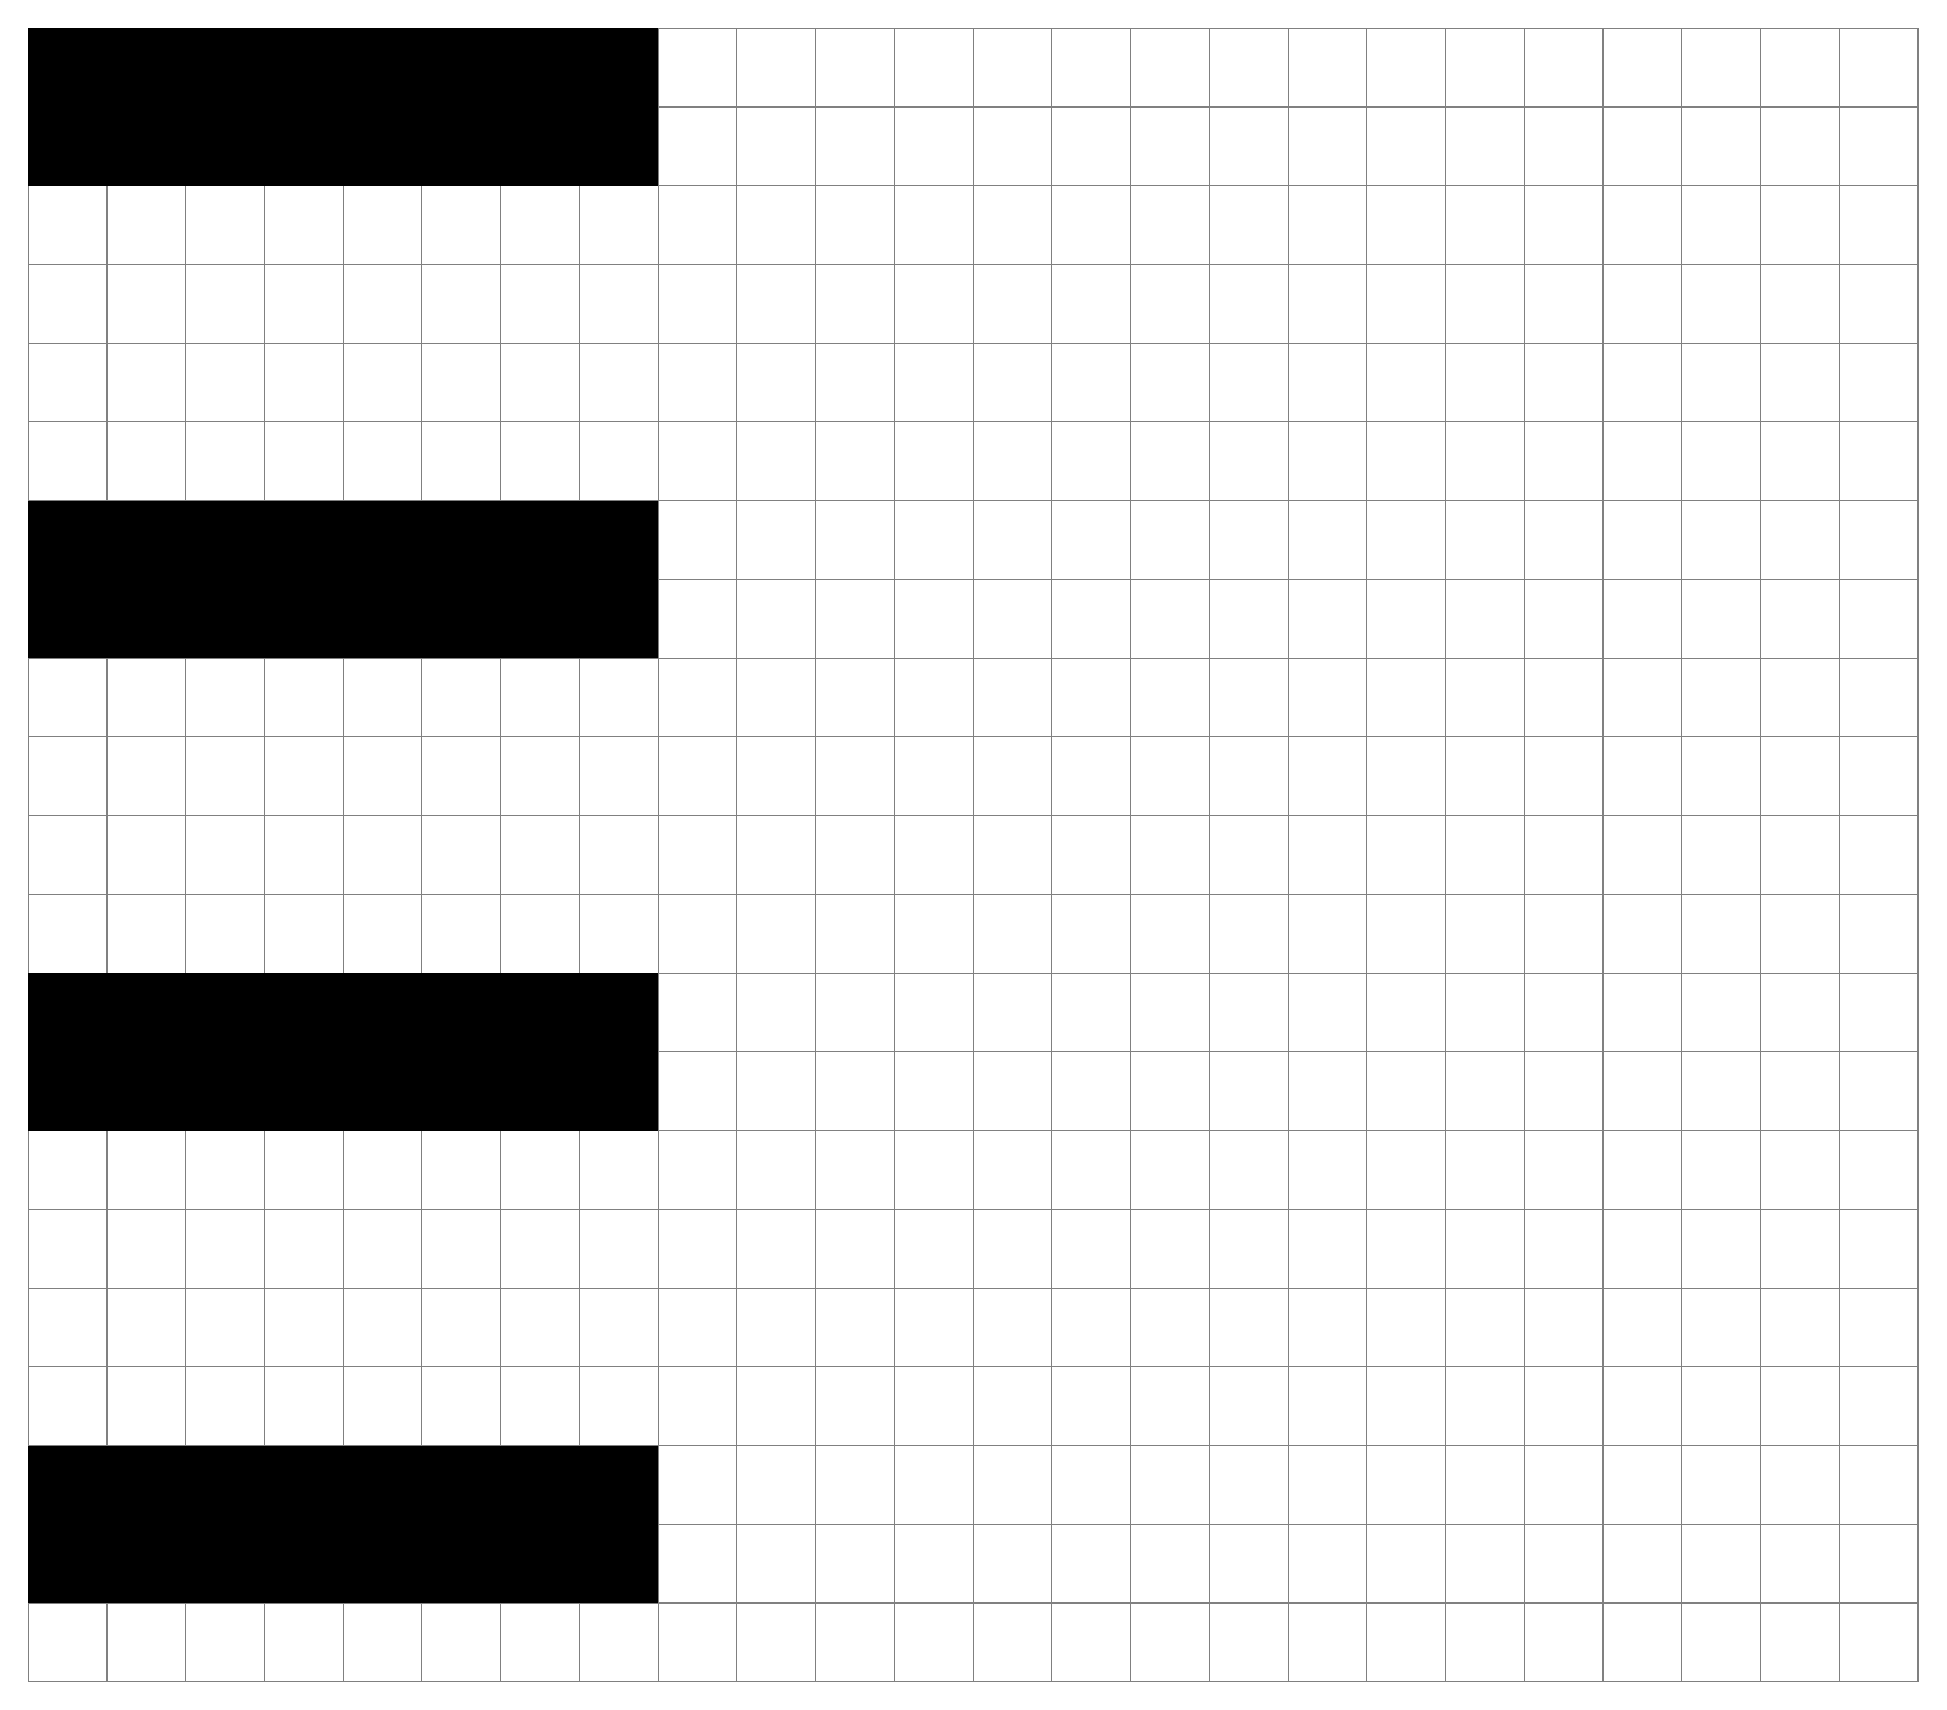
\begin{tikzpicture}

	\draw[step=1.0,gray,thin] (0,0) grid (24,21);
	\fill[\MULTICOLORTWO] (0,20) rectangle ++ (1,1);
	\fill[\MULTICOLORTWO] (1,20) rectangle ++ (1,1);
	\fill[\MULTICOLORTWO] (2,20) rectangle ++ (1,1);
	\fill[\MULTICOLORTWO] (3,20) rectangle ++ (1,1);
	\fill[\MULTICOLORTWO] (4,20) rectangle ++ (1,1);
	\fill[\MULTICOLORTWO] (5,20) rectangle ++ (1,1);
	\fill[\SPRITECOLOR] (6,20) rectangle ++ (1,1);
	\fill[\SPRITECOLOR] (7,20) rectangle ++ (1,1);
	\fill[\MULTICOLORTWO] (0,19) rectangle ++ (1,1);
	\fill[\MULTICOLORTWO] (1,19) rectangle ++ (1,1);
	\fill[\MULTICOLORTWO] (2,19) rectangle ++ (1,1);
	\fill[\MULTICOLORTWO] (3,19) rectangle ++ (1,1);
	\fill[\MULTICOLORTWO] (4,19) rectangle ++ (1,1);
	\fill[\MULTICOLORTWO] (5,19) rectangle ++ (1,1);
	\fill[\SPRITECOLOR] (6,19) rectangle ++ (1,1);
	\fill[\SPRITECOLOR] (7,19) rectangle ++ (1,1);
	\fill[\MULTICOLORTWO] (0,14) rectangle ++ (1,1);
	\fill[\MULTICOLORTWO] (1,14) rectangle ++ (1,1);
	\fill[\MULTICOLORTWO] (2,14) rectangle ++ (1,1);
	\fill[\MULTICOLORTWO] (3,14) rectangle ++ (1,1);
	\fill[\MULTICOLORTWO] (4,14) rectangle ++ (1,1);
	\fill[\MULTICOLORTWO] (5,14) rectangle ++ (1,1);
	\fill[\SPRITECOLOR] (6,14) rectangle ++ (1,1);
	\fill[\SPRITECOLOR] (7,14) rectangle ++ (1,1);
	\fill[\MULTICOLORTWO] (0,13) rectangle ++ (1,1);
	\fill[\MULTICOLORTWO] (1,13) rectangle ++ (1,1);
	\fill[\MULTICOLORTWO] (2,13) rectangle ++ (1,1);
	\fill[\MULTICOLORTWO] (3,13) rectangle ++ (1,1);
	\fill[\MULTICOLORTWO] (4,13) rectangle ++ (1,1);
	\fill[\MULTICOLORTWO] (5,13) rectangle ++ (1,1);
	\fill[\SPRITECOLOR] (6,13) rectangle ++ (1,1);
	\fill[\SPRITECOLOR] (7,13) rectangle ++ (1,1);
	\fill[\MULTICOLORTWO] (0,8) rectangle ++ (1,1);
	\fill[\MULTICOLORTWO] (1,8) rectangle ++ (1,1);
	\fill[\MULTICOLORTWO] (2,8) rectangle ++ (1,1);
	\fill[\MULTICOLORTWO] (3,8) rectangle ++ (1,1);
	\fill[\MULTICOLORTWO] (4,8) rectangle ++ (1,1);
	\fill[\MULTICOLORTWO] (5,8) rectangle ++ (1,1);
	\fill[\SPRITECOLOR] (6,8) rectangle ++ (1,1);
	\fill[\SPRITECOLOR] (7,8) rectangle ++ (1,1);
	\fill[\MULTICOLORTWO] (0,7) rectangle ++ (1,1);
	\fill[\MULTICOLORTWO] (1,7) rectangle ++ (1,1);
	\fill[\MULTICOLORTWO] (2,7) rectangle ++ (1,1);
	\fill[\MULTICOLORTWO] (3,7) rectangle ++ (1,1);
	\fill[\MULTICOLORTWO] (4,7) rectangle ++ (1,1);
	\fill[\MULTICOLORTWO] (5,7) rectangle ++ (1,1);
	\fill[\SPRITECOLOR] (6,7) rectangle ++ (1,1);
	\fill[\SPRITECOLOR] (7,7) rectangle ++ (1,1);
	\fill[\MULTICOLORTWO] (0,2) rectangle ++ (1,1);
	\fill[\MULTICOLORTWO] (1,2) rectangle ++ (1,1);
	\fill[\MULTICOLORTWO] (2,2) rectangle ++ (1,1);
	\fill[\MULTICOLORTWO] (3,2) rectangle ++ (1,1);
	\fill[\MULTICOLORTWO] (4,2) rectangle ++ (1,1);
	\fill[\MULTICOLORTWO] (5,2) rectangle ++ (1,1);
	\fill[\SPRITECOLOR] (6,2) rectangle ++ (1,1);
	\fill[\SPRITECOLOR] (7,2) rectangle ++ (1,1);
	\fill[\MULTICOLORTWO] (0,1) rectangle ++ (1,1);
	\fill[\MULTICOLORTWO] (1,1) rectangle ++ (1,1);
	\fill[\MULTICOLORTWO] (2,1) rectangle ++ (1,1);
	\fill[\MULTICOLORTWO] (3,1) rectangle ++ (1,1);
	\fill[\MULTICOLORTWO] (4,1) rectangle ++ (1,1);
	\fill[\MULTICOLORTWO] (5,1) rectangle ++ (1,1);
	\fill[\SPRITECOLOR] (6,1) rectangle ++ (1,1);
	\fill[\SPRITECOLOR] (7,1) rectangle ++ (1,1);

      \end{tikzpicture}
    \end{adjustbox}
  }\caption{STARFIELD\_SPRITE}
\end{figure}
